% Chapter 1
\chapter{مقدمه}

\section{اهمیت مسئله}
برای پانویس شدن و همچنین درج کلمه در فهرست کلمات، علامت * را در هنگام فراخوانی دستور دیکشنری حذف کنید. در عناوین بخش ها و چکیده نباید پانویس شود.

  
\section{ساختار گزارش}

این یک متن نمونه است... این یک متن نمونه است...این یک متن نمونه است...این یک متن نمونه است...این یک متن نمونه است...این یک متن نمونه است...این یک متن نمونه است...این یک متن نمونه است...این یک متن نمونه است...این یک متن نمونه است...این یک متن نمونه است... این یک متن نمونه است...این یک متن نمونه است...این یک متن نمونه است...این یک متن نمونه است...این یک متن نمونه است...این یک متن نمونه است...این یک متن نمونه است...این یک متن نمونه است...این یک متن نمونه است...این یک متن نمونه است... این یک متن نمونه است...این یک متن نمونه است...این یک متن نمونه است...این یک متن نمونه است...این یک متن نمونه است...این یک متن نمونه است...این یک متن نمونه است...این یک متن نمونه است...این یک متن نمونه است...این یک متن نمونه است... این یک متن نمونه است...این یک متن نمونه است...این یک متن نمونه است...این یک متن نمونه است...این یک متن نمونه است...
اینگونه به شکل رفرنس دهید (شکل \ref{fig:intro:populationpyramid} را ببینید)، 
‎\begin{figure}[t!]‎
	\centering
	\subfloat[‏]{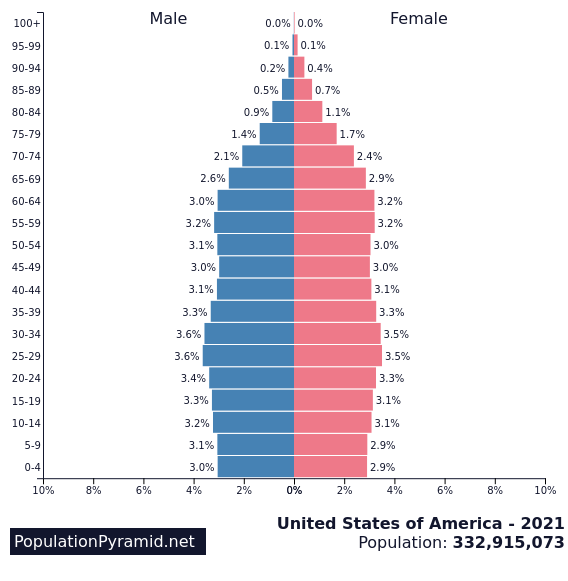
\includegraphics[width=7.25cm]{images/population_data/USA.png}}
	\qquad
	\subfloat[]{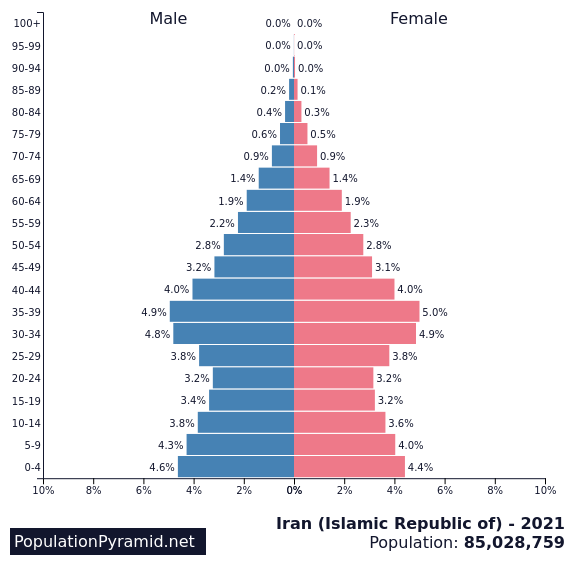
\includegraphics[width=7.25cm]{images/population_data/iran.png}}
	\caption[عنوان شکل در فهرست اشکال]
	{مقایسه هرم جمعیتی دو کشور (الف) ایران و (ب) آمریکا }
	\label{fig:intro:populationpyramid}
\end{figure} 

این یک متن نمونه است...این یک متن نمونه است...این یک متن نمونه است...این یک متن نمونه است...این یک متن نمونه است... این یک متن نمونه است...این یک متن نمونه است...این یک متن نمونه است...این یک متن نمونه است...این یک متن نمونه است...این یک متن نمونه است...این یک متن نمونه است...این یک متن نمونه است...این یک متن نمونه است... 
اینگونه رفرنس بدهید \cite{karimi2020soft, mohammadimohammadabadi}. 


